\chapter{GUI Windows}

%-----------------------------------------------------------------
\section{The Main GUI Window}
\label{s:gui.root.window}

The main window for the GUI is shown in Figure \ref{fig:root.window}.
\begin{figure}
\centering
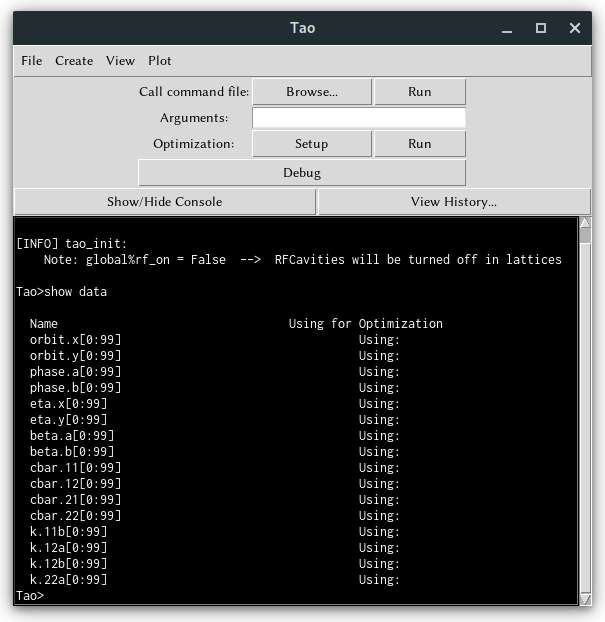
\includegraphics[width=8cm]{figures/root_window.png}
\caption{The main GUI window, showing the results of \texttt{show data} on the console.}
\label{fig:root.window}
\end{figure}
From here, the user has access to all of the GUI's features.
Command files can be called by browsing for them and then clicking "Run", with arguments specified in the "Arguments" below.
In the future, the user will also be able to set up and run optimization routines from this window, although this feature is not currently available.

The main window also has a console, where commands can be run in Tao exactly like in regular Tao.
The console will also display warning messages if a command produces an error.

%-----------------------------------------------------------------
\section{Global Variables}
\label{s:gui.global.variables}

Global variables in Tao can be viewed and modified from the global variables window as shown in Figure \ref{fig:gui.global.variables}.
Once you have editted the global variables, clicking the "Set Global Variables" button will set the variables in Tao as appropriate.

\begin{figure}
\centering
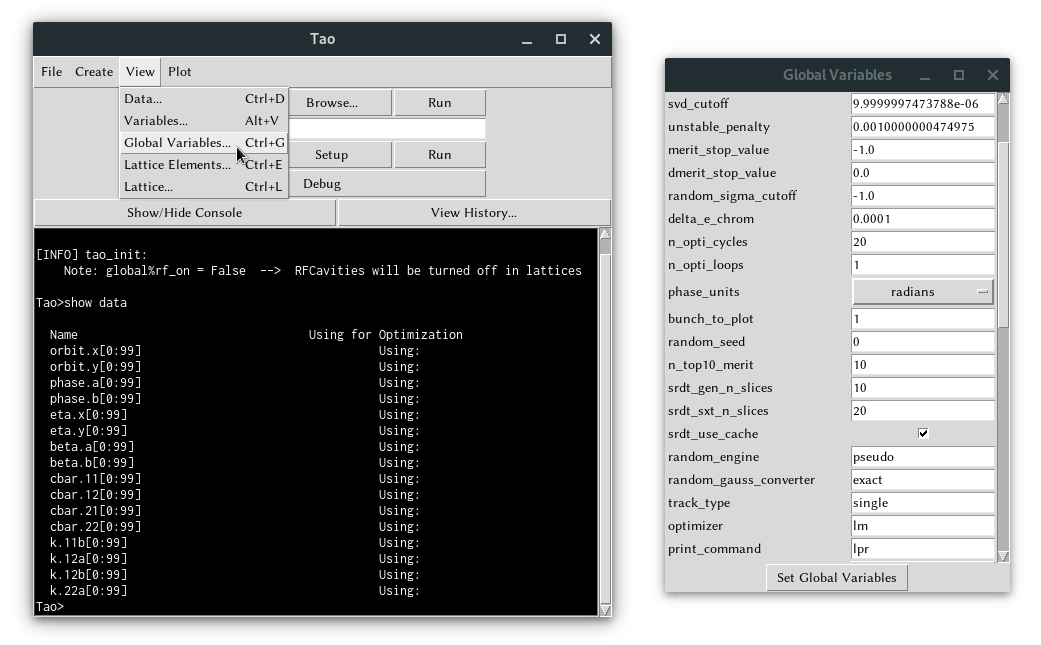
\includegraphics[width=10cm]{figures/globals.png}
\caption{View and edit global variables with the Global Variables window.}
\label{fig:gui.global.variables}
\end{figure}

%-----------------------------------------------------------------
\section{Data}
\label{s:gui.data}

The GUI provides several windows for viewing and editing data arrays.

\subsection{Viewing Data}
\label{s:gui.data.view}

Figure \ref{fig:gui.data.view} shows the various windows that the GUI provides for viewing data and making minor changes to data arrays.
\begin{figure}
\centering
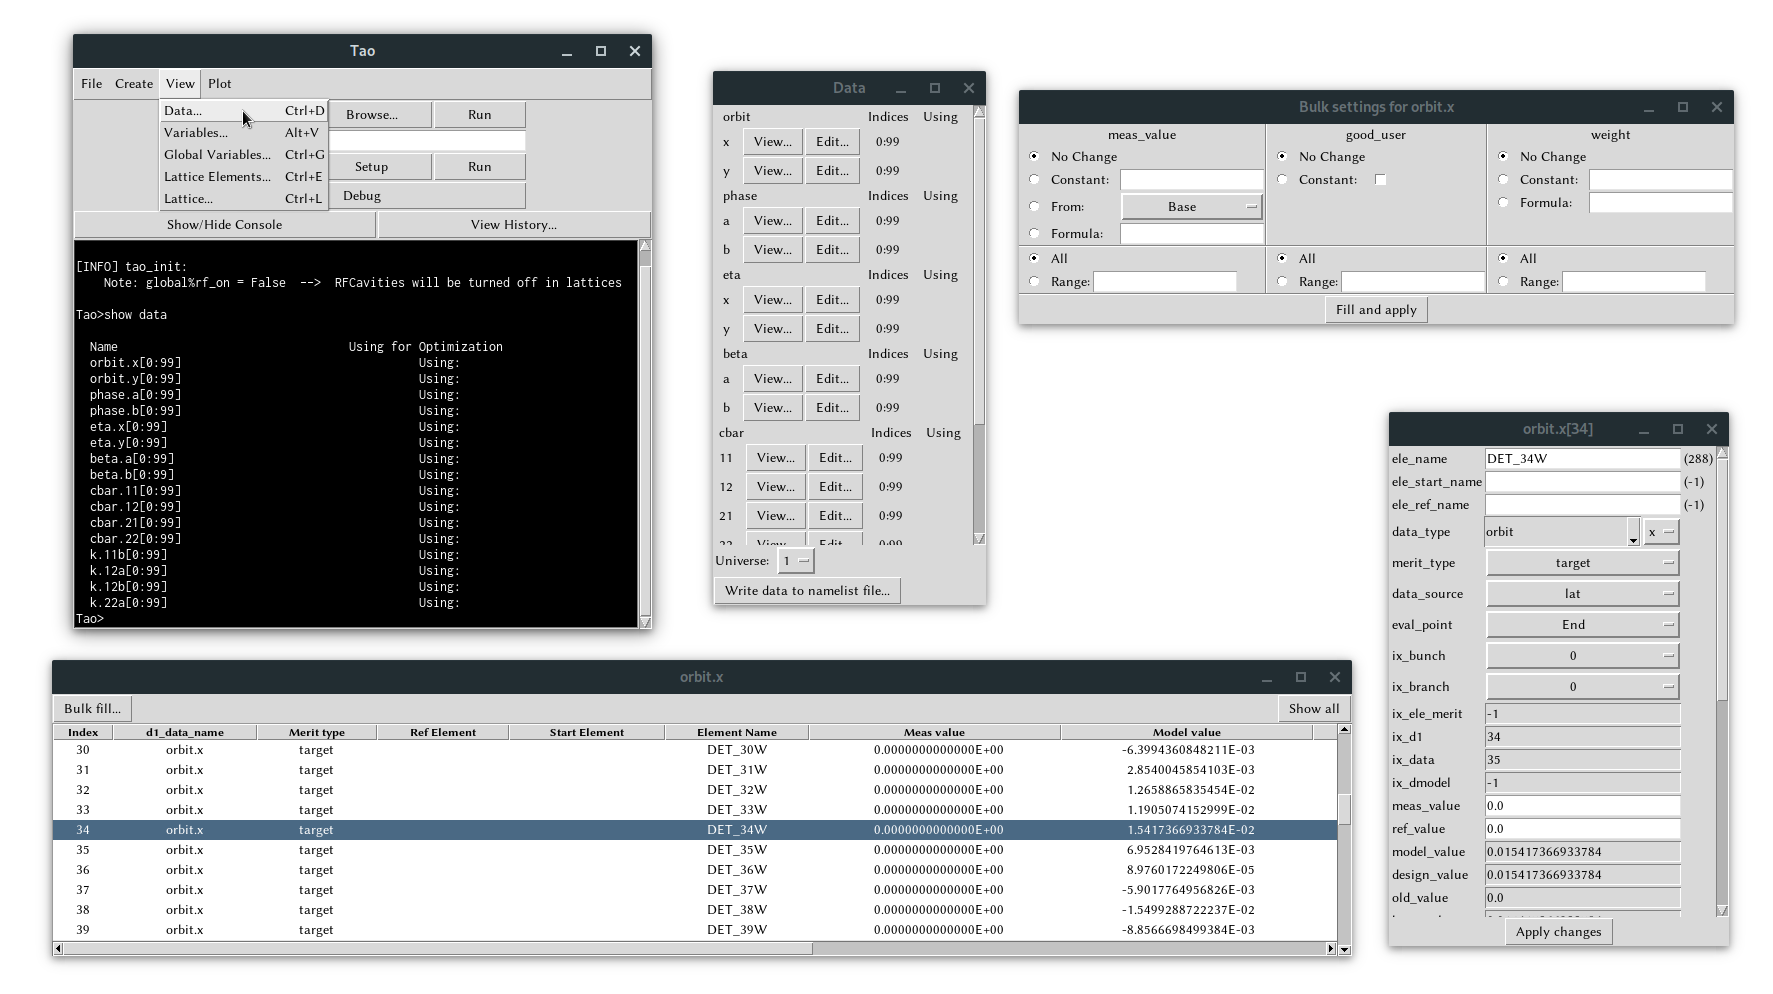
\includegraphics[width=12cm]{figures/view_data.png}
\caption{The GUI's data viewing windows.
Top left: the Tao root window and the menu shortcut for viewing data.
Top middle: The d2_data_array window, which list the currently defined d2_data_arrays for each universe.
This window also includes links to view and edit (see section \ref{s:gui.data.edit}) existing d1_data_arrays.
Bottom left: The d1_data_array window (in this case for orbit.x), showing all of the datums in the array orbit.x.
Bottom right: The individual datum window (in this case for orbit.x[34]) displaying detailed datum properties and allowing the user to edit some of these properties.
Top right: The bulk edit window (in this case for orbit.x) providing controls to quickly edit a few key properties for multiple datums in a d1_data_array.}
\label{fig:gui.data.view}
\end{figure}

The d2_data_array window (top middle in Figure \ref{fig:gui.data.view}) displays all data arrays for a given universe.
To view any existing d1_data_array, click on its "View" button.
This window also provides the ability to edit any existing data array in detail (see Section \ref{s:gui.data.edit}), as well as functionality for writing existing data to a namelist (see Section \ref{s:gui.namelist}).

The d1_data_array window (bottom left in Figure \ref{fig:gui.data.view}) allows the user to view an existing d1_data_array.
This window displays important properties of each datum in the array, such as element name, meas, model, and design values, and weight, in a scrollable table.
To view a datum in detail, double click on its row in the d1_data_array window.
This will open the individual datum window for that datum, displaying all of its properties and allowing some of them to be editted.

The d1_data_array window also allows the user to edit a few key properties of the datums in the array all at once using the bulk settings window (top right in Figure \ref{fig:gui.data.view}).
This window is accessed by clicking on the "Bulk fill" button in the d1_data_array window.
From here, the meas_value, good_user, and weight settings for the datums in the array can be edited in bulk.
Changes may be applied to every datum in the array, or to only a specific range of datums using the range specifier.
Once the desired settings have been specified, clicking the "Fill and apply" button will edit the d1_data_array as necessary, and changes will be reflected in the d1_data_array window.

\subsection{Creating and Editing Data}
\label{s:gui.data.edit}

The GUI also supports the creation of data arrays on the fly through the create data window.
This window can be accessed as shown in figure \ref{fig:gui.create.data.d2}.
\begin{figure}
\centering
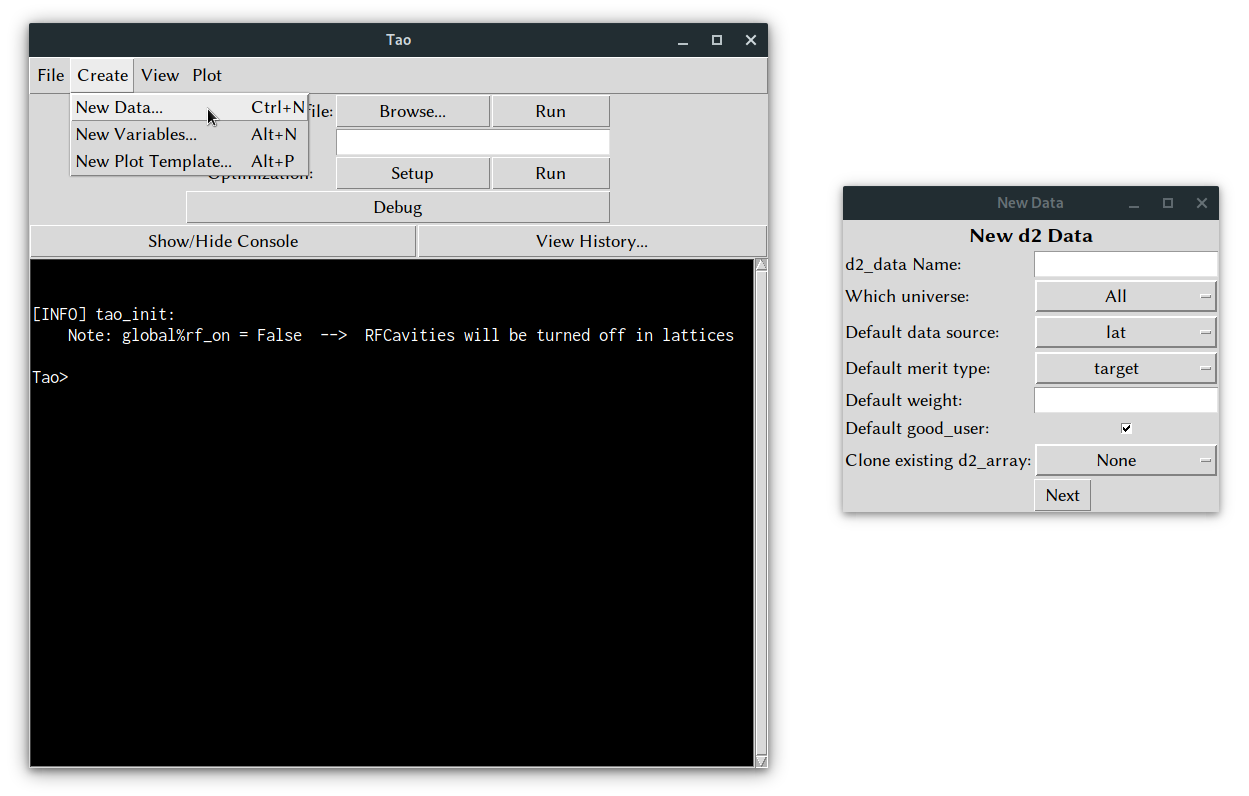
\includegraphics[width=12cm]{figures/create_d2.png}
\caption{Left: the data creation window can be accessed from the root window's menubar. \\
Right: The first pane of the data creation window.}
\label{fig:gui.create.data.d2}
\end{figure}
In the first pane of the data creation window, the user can input the desired settings for the new d2_data_array.
The user can also select and existing d2_data_array to clone.
This will copy the d2 properties of that array, as well as the d1 properties and all of the datums for each d1 array.
Once this information has been input, the user can hit the "Next" button to go to the d1_data_array pane.

The d1_array pane of the data creation window is where most of the data array's properties are set.
This pane is shown in Figure \ref{fig:gui.create.data.d1}.
\begin{figure}
\centering
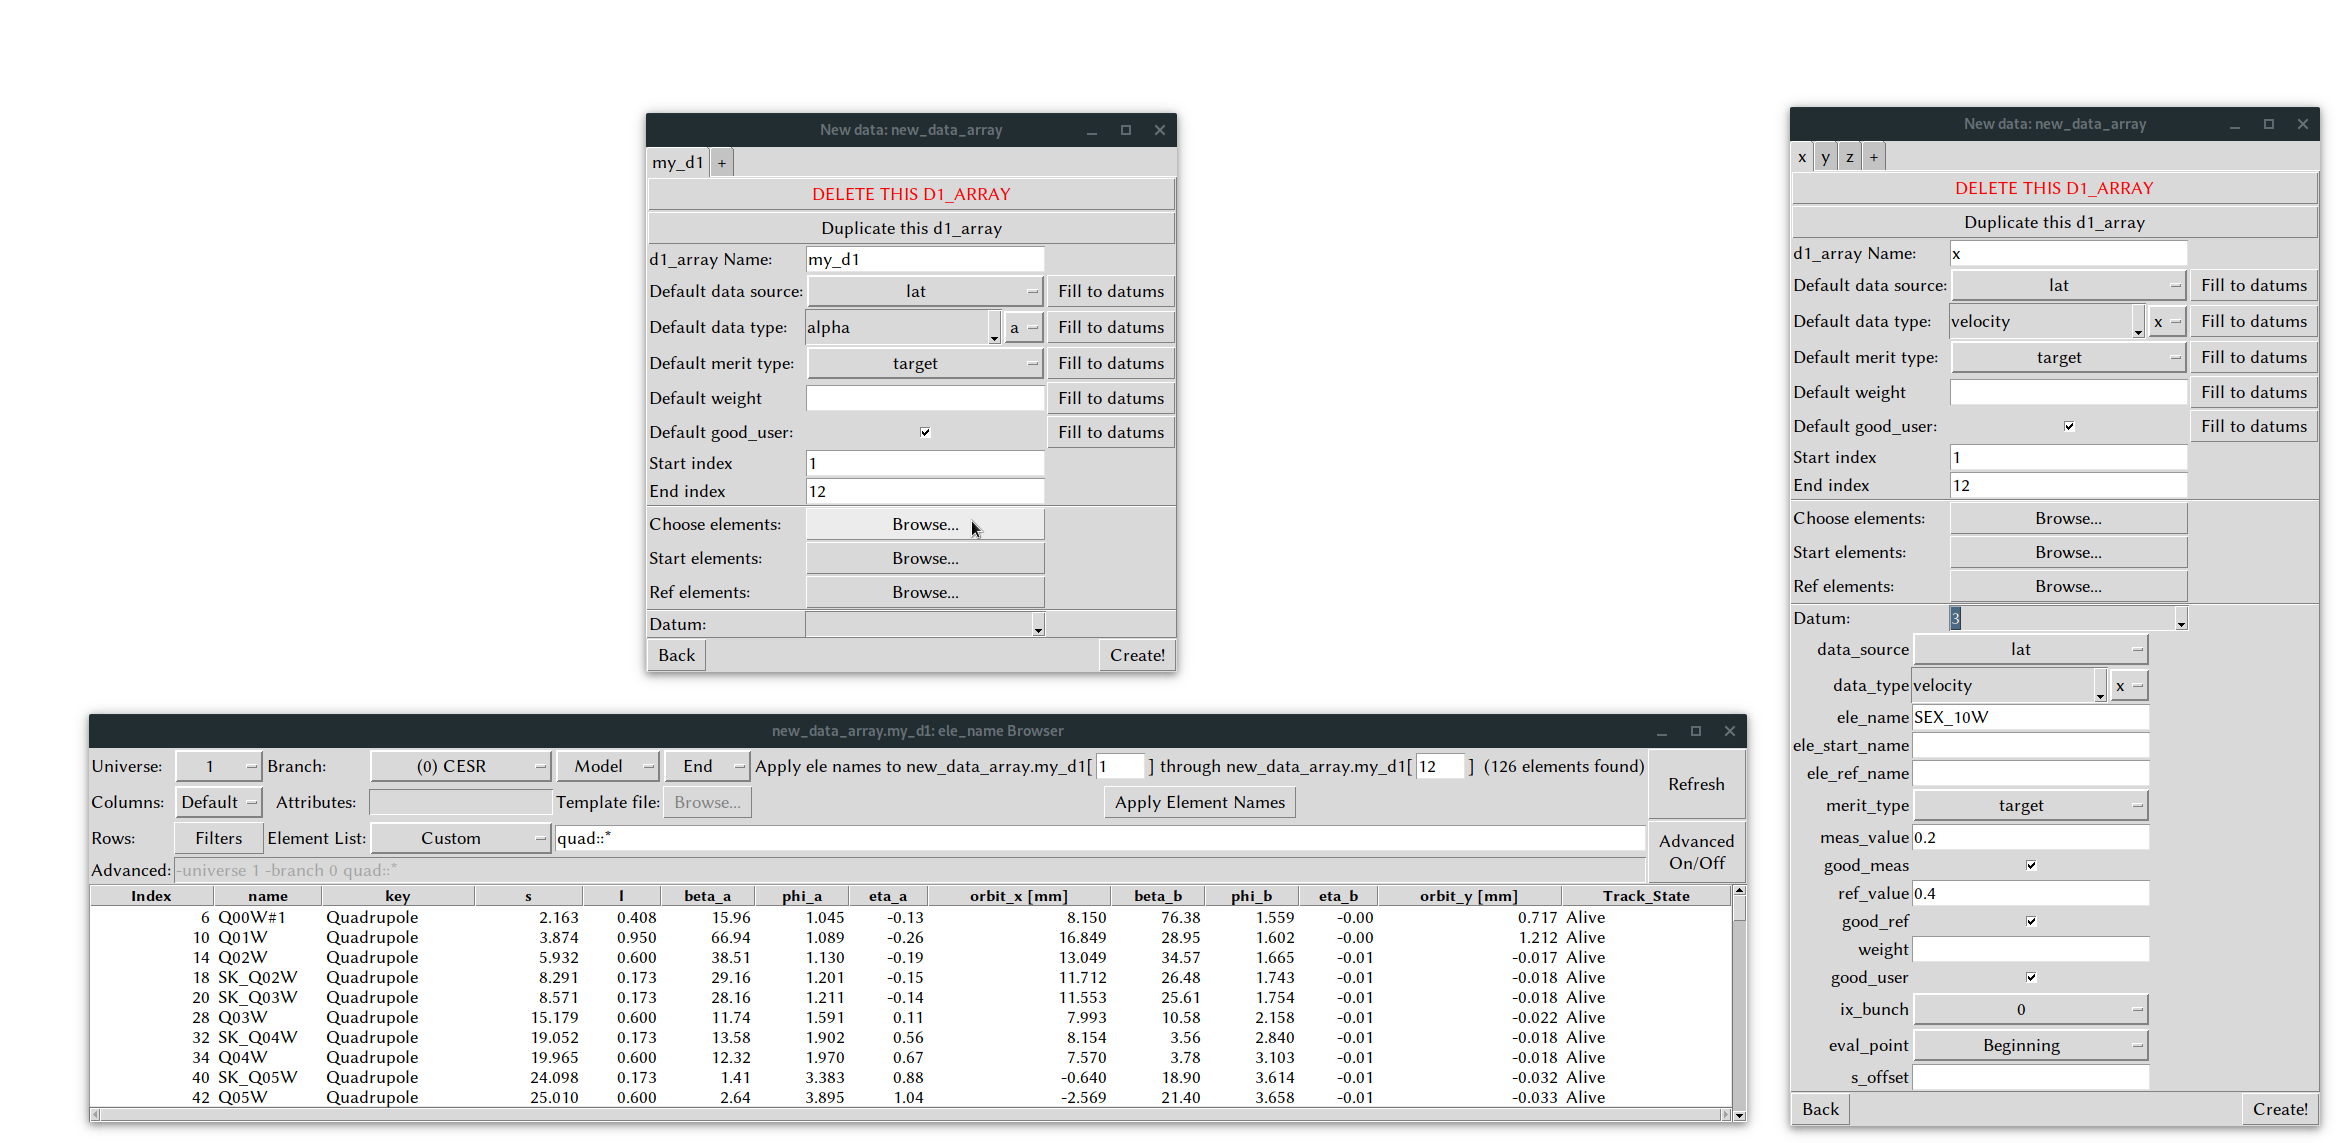
\includegraphics[width=12cm]{figures/create_d1.png}
\caption{The d1_array pane of the data creation window.  Top left: Here, only one d1_array has been created (called my_d1), its default data type has been set to alpha.a, and the start and end indices have been set to 1 and 12 respectively.  \\
Bottom left: the lattice browser for the ele_names that will be used with my_d1.
Right: Here, the user has defined three d1_arrays: x, y, and z.
The data type for new_data_array.x has been set to velocity.x, and the start and end indices have been set to 1 and 12.
Here, the user is currently editing new_data_array.x[3], where the meas value has been set to 0.2 and the ref value has been set to 0.4.}
\label{fig:gui.create.data.d1}
\end{figure}
The d1_array pane of the data creation window displays each d1_array in its own tab.
To add a tab, click on the "+" tab at the top of the window.
Tabs can also be removed by navigating to them and then clicking on their delete button.
An existing tab can also be duplicated by clicking on the duplicate button right under the delete button.
This may be useful if you want to define several d1_arrays with many of the same properties, but want them each to have a different data type, for example.

The next section of the window holds the d1-level settings for the array.
Here, the d1 name, start index, and end index can be set, as well as the default data_source, data_type, merit type, weight, and good user value for the d1_array.

The next section allows the users to set the ele_name, ele_start_name, and ele_ref_name for the d1_array en-masse.
Clicking on these buttons will bring up the lattice browser window (bottom left in Figure \ref{fig:gui.create.data.d1}).
This window is essentially identical to the main lattice window for the GUI (see Section \ref{s:gui.lat}), with a few additions.
Towards the top right of the window, the user can specify which indices to read the element names into.
Clicking "Apply Element Names" will then write the ele names that are currently in the table sequentially into the d1_array's datums.
In the example shown in Figure \ref{fig:gui.create.data.d1}, new_data_array.my_d1[1]|ele_name will be set to "Q00W\#1", new_data_array.my_d1[2]|ele_name will be set to "Q01W", and so on.
If there are more elements in the table than there are datums to write to, the table will be truncated and only the first elements in the table will be used.
If there are less elements in the table than there are datums to write to, the elements in the table will be looped through so that each datum gets an element name.

The bottom portion of the d1_array pane of the data creation window allows the user to set the properties of the individual datums in the array.
Once a start and end index have been specified, the "Datum" drop down menu will be populated with all of the datum indices.
Selecting an index will bring up the datum settings for that datum, as shown in the right of Figure \ref{fig:gui.create.data.d1}.
Note that any settings that have a d1-level default value are automatically filled in.
Once the user edits a property of a datum, that property will no longer be auto-filled from the d1-level default settings, even if those default values are subsequently edited.
If the user wants to explicitly fill a d1 setting to that d1_array's datums, they may do so with the corresponding "Fill to datums" button.

Once all of the data settings have been adjusted as necessary, the user must click the "Create" button to create the d2_array in Tao.  Doing so will close the data creation window.

The data creation window can also be accessed from the d2_data window discussed in Section \ref{s:gui.data.view}.
Clicking on the "Edit" button for any d2 array will load that array into the data creation window, just as if the user had cloned that array from the d2 pane of the data creation window.
This is shown in Figure \ref{fig:gui.edit.data}
\begin{figure}
\centering
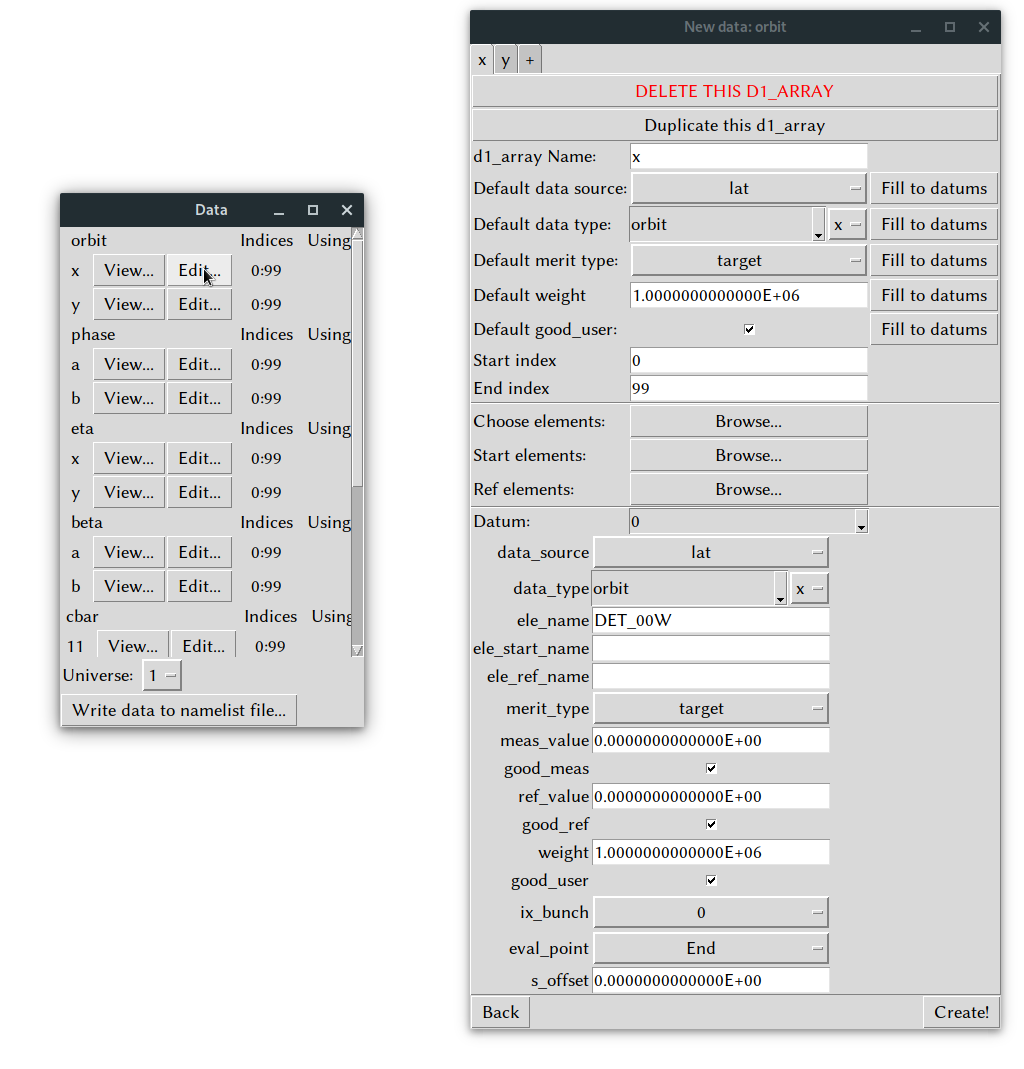
\includegraphics[width=12cm]{figures/edit_data.png}
\caption{Editting an existing d2_data_array.}
\label{fig:gui.edit.data}
\end{figure}
Note that any changes made in the data creation window will not take effect in Tao until the user clicks the "Create" button.
For example, clicking the delete button for the orbit.x array would not actually delete the array in Tao until the user clicks "Create".

%-----------------------------------------------------------------
\section{Variables}
\label{s:gui.variables}

Variables are viewed and edited in the GUI almost exactly the same as data, as shown in Figure \ref{fig:gui.variables}.
\begin{figure}
\centering
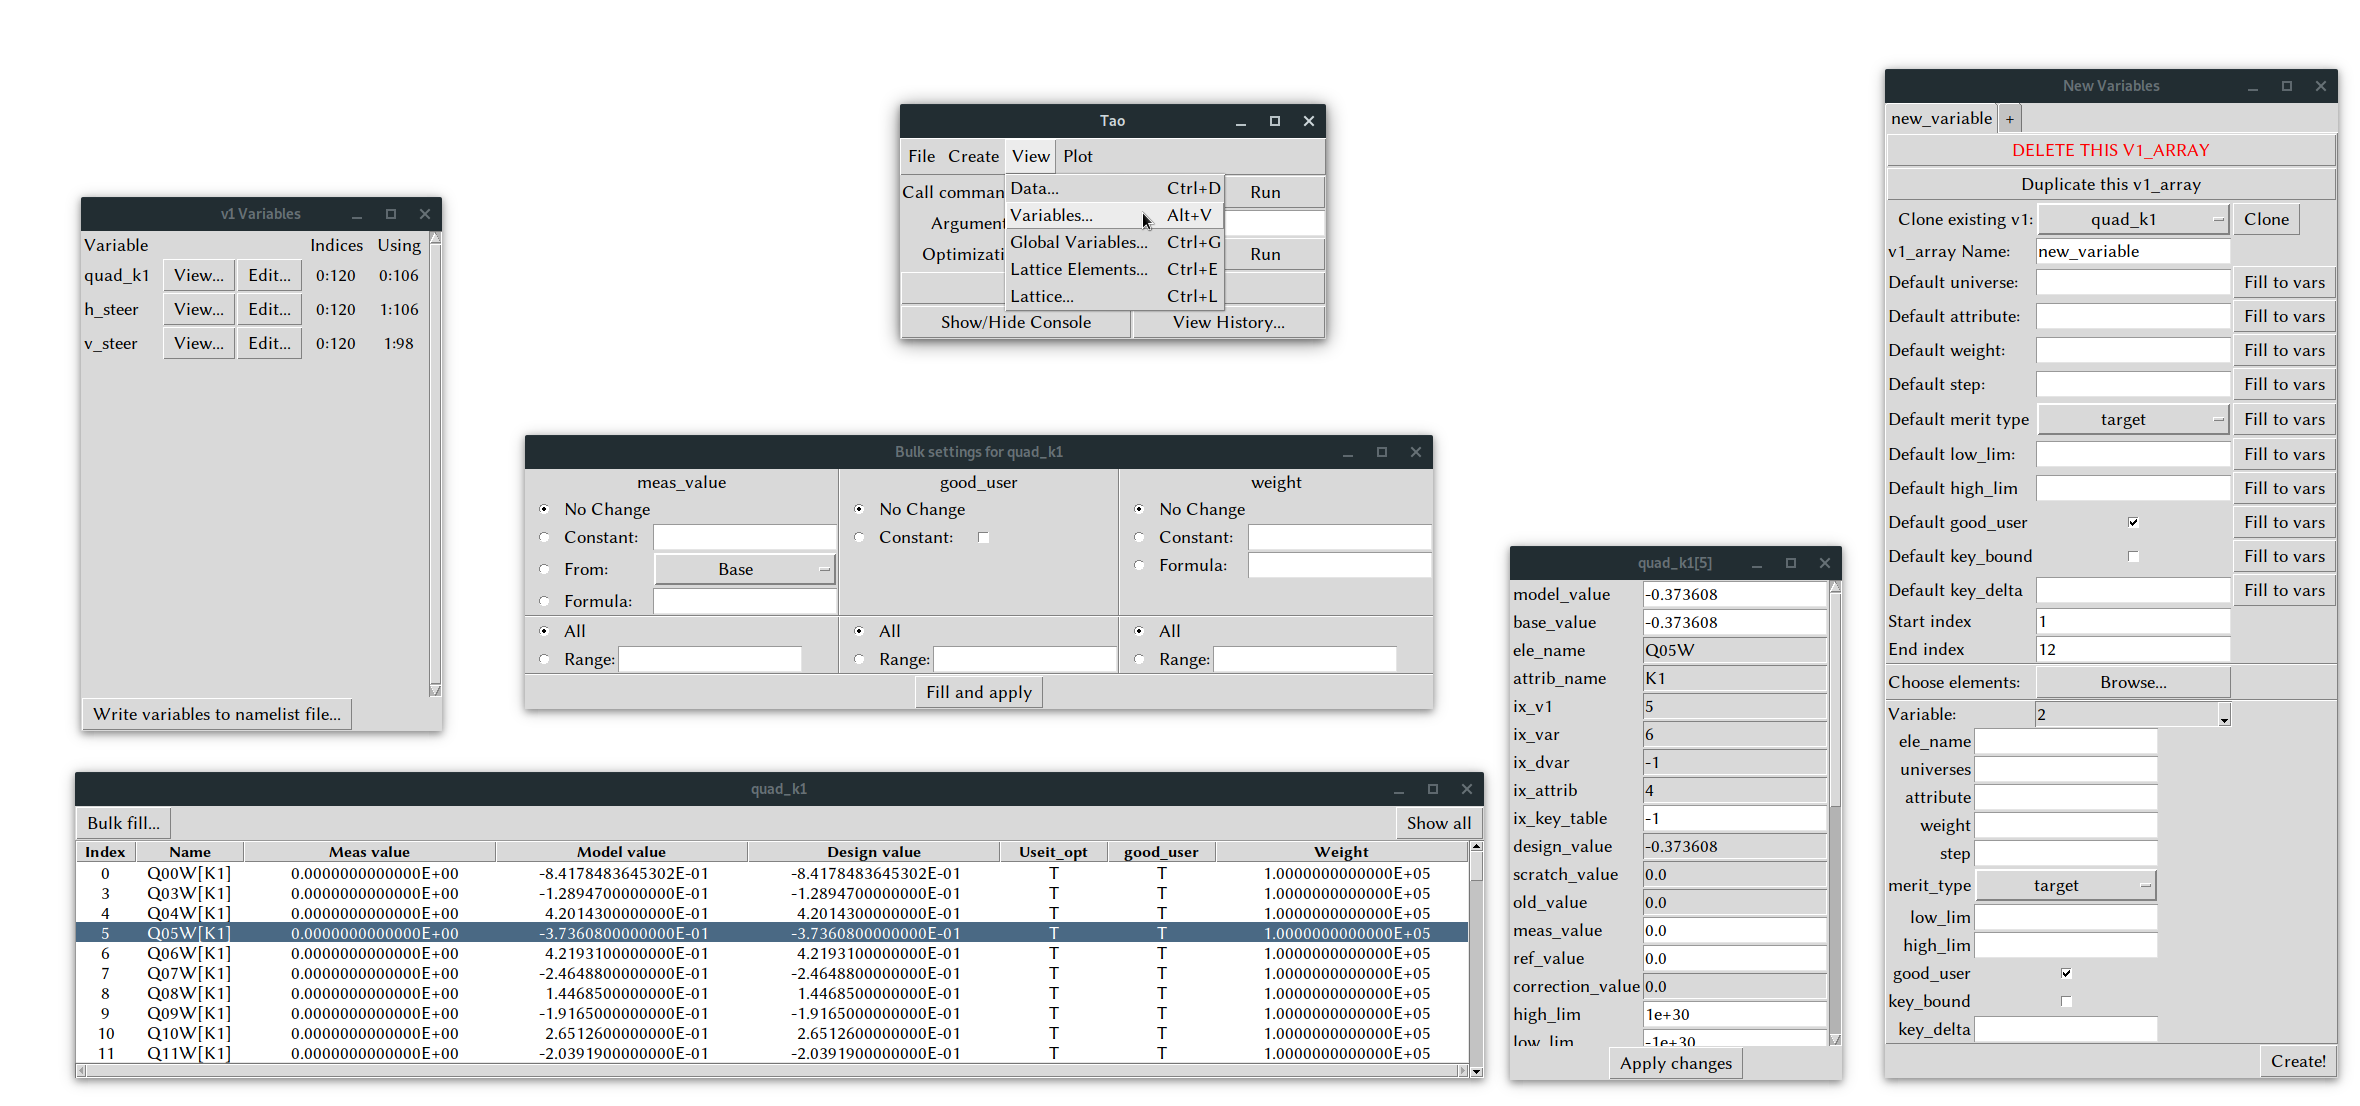
\includegraphics[width=12cm]{figures/variables.png}
\caption{The variable viewing and editing windows in the GUI.
Top middle: accessing the v1 variable window from the root window (console hidden).
Top left: the v1 variable window, showing the currently defined v1 variable arrays.
Bottom left: the variable window for quad_k1, displaying each of its variables and their key attributes.
Middle: the bulk fill window for quad_k1.
Bottom middle: the individual variable window for quad_k1[5], showing all of its settings and allowing the user to edit some of them.
Right: The variable array creation window.}
\label{fig:gui.variables}
\end{figure}
An important exception is that, since there are only v1 variables arrays and no v2 arrays of v1 arrays, the variable creation window only has one pane, and separate v1 arrays created in different tabs of the window are completely independent.
Also, the user can clone an existing v1 array with the drop down menu below the "Duplicate" button.

%-----------------------------------------------------------------
\section{Plotting}
\label{s:gui.plot}

One of the GUI's strong suits is the ability to view an manipulate plots using matplotlib.
Existing plots can be viewed and edited, and new templates can be defined on the fly.

Note: the GUI does support classic PG/PLplots, but it is recommended to use matplotlib as the plotting engine due to the extra fatures it offers.

\subsection{Viewing Plots}
\label{s:gui.plot.view}
Figure \ref{fig:gui.plot.view} shows how to plot existing templates in the GUI.
\begin{figure}
\centering
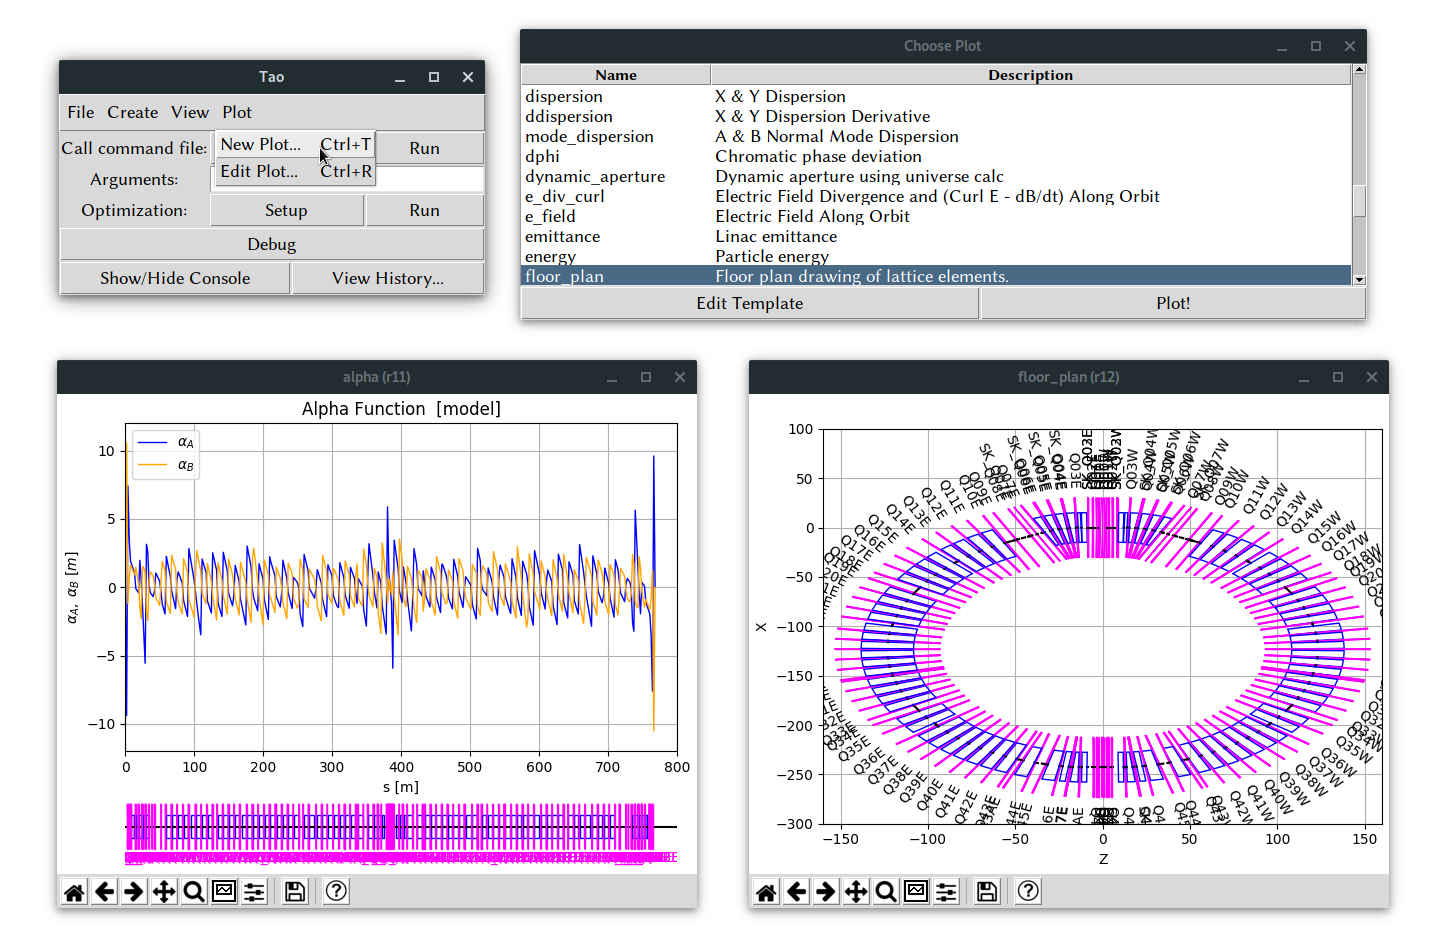
\includegraphics[width=12cm]{figures/view_plot.png}
\caption{Viewing plots with the GUI.
Top left: accessing the plot template list from the root window.
Top right: the plot template window.
Bottom left: a plot of the alpha function with the lat_layout shown below.
Bottom right: the floor_plan plot.}
\label{fig:gui.plot.view}
\end{figure}
The plot template window lists all of the currently defined plot templates as well as their descriptions.
A template can be plotted either by double clicking on it, or by selecting it and then clicking the "Plot" button.
This will open a window displaying the selected plot (see Section \ref{s:gui.plot.interaction} for more information).
The user can also edit an existing template by selecting it in the tempalte window and clicking "Edit Template".


\subsection{Interacting with Plots}
\label{s:gui.plot.interaction}
Interacting with plots in the GUI is primarily done using the toolbar along the bottom of the plotting window.

Starting from the left, the home button returns the graph to the starting view. The back button returns to the previous view of the graph, working as an undo button. The forward button undoes the effects of the back button. All of these buttons also have keyboard shortcuts, 'h' or 'r' for home, 'c' or 'left arrow' for back, and 'v' or 'right arrow' for forward.

The pan/zoom button allows panning of the graph by holding a left click on the graph and dragging the mouse around. his mode also allows zooming of the graph by holding a right click on the graph and dragging the mouse around. These actions can be restricted to the horizontal axis by holding 'x' while dragging, or the vertical axis by holding 'y'. Holding 'control' while dragging the mouse will preserve aspect ratio. Clicking on the toolbar button again will get out of this mode.

The zoom to rectangle button allows a rectangle to be selected by holding a left click on the graph and dragging the mouse, which will then fill the graph window. Holding 'x' or 'y' while selecting a rectangle will only effect the horizontal or vertical axis respectively.

The save button allows the graph window to be saved as an image file. Using 'ctrl+s' has the same effect.

If any floor plan or lat layout is present, double clicking on an element will open a window to view or edit element parameters.

Floor plans contain a slider to scale the size of elements away from the element centerline. Clicking on the slider will adjust the width of the displayed elements.

%-----------------------------------------------------------------
\subsection{Plotting Initialization}
\label{s:gui.plot.init}

When operating the GUI in matplotlib mode, you can specify a list of template plots to plot in matplotlib as soon as tao starts.  These templates should be listed in a file called plot.gui.init, which should be in the same directory from which you launch the gui.

plot.gui.init should have one template listed per line and absolutely nothing else on the line.  The templates listed in plot.gui.init are checked against the list of templates that tao can plot, and if a template is not recognized it is simply ignored.


%-----------------------------------------------------------------
\section{Lattice Elements}
\label{s:gui.lat}

The GUI provides the ability to view and edit the elements of a lattice through the lattice table window and through the element browser.

\subsection{Viewing the Lattice}
\label{s:gui.lat.table}

The primary window for viewing the lattice is the lattice table window, as shown in Figure \ref{fig:gui.lat.table}.
\begin{figure}
\centering
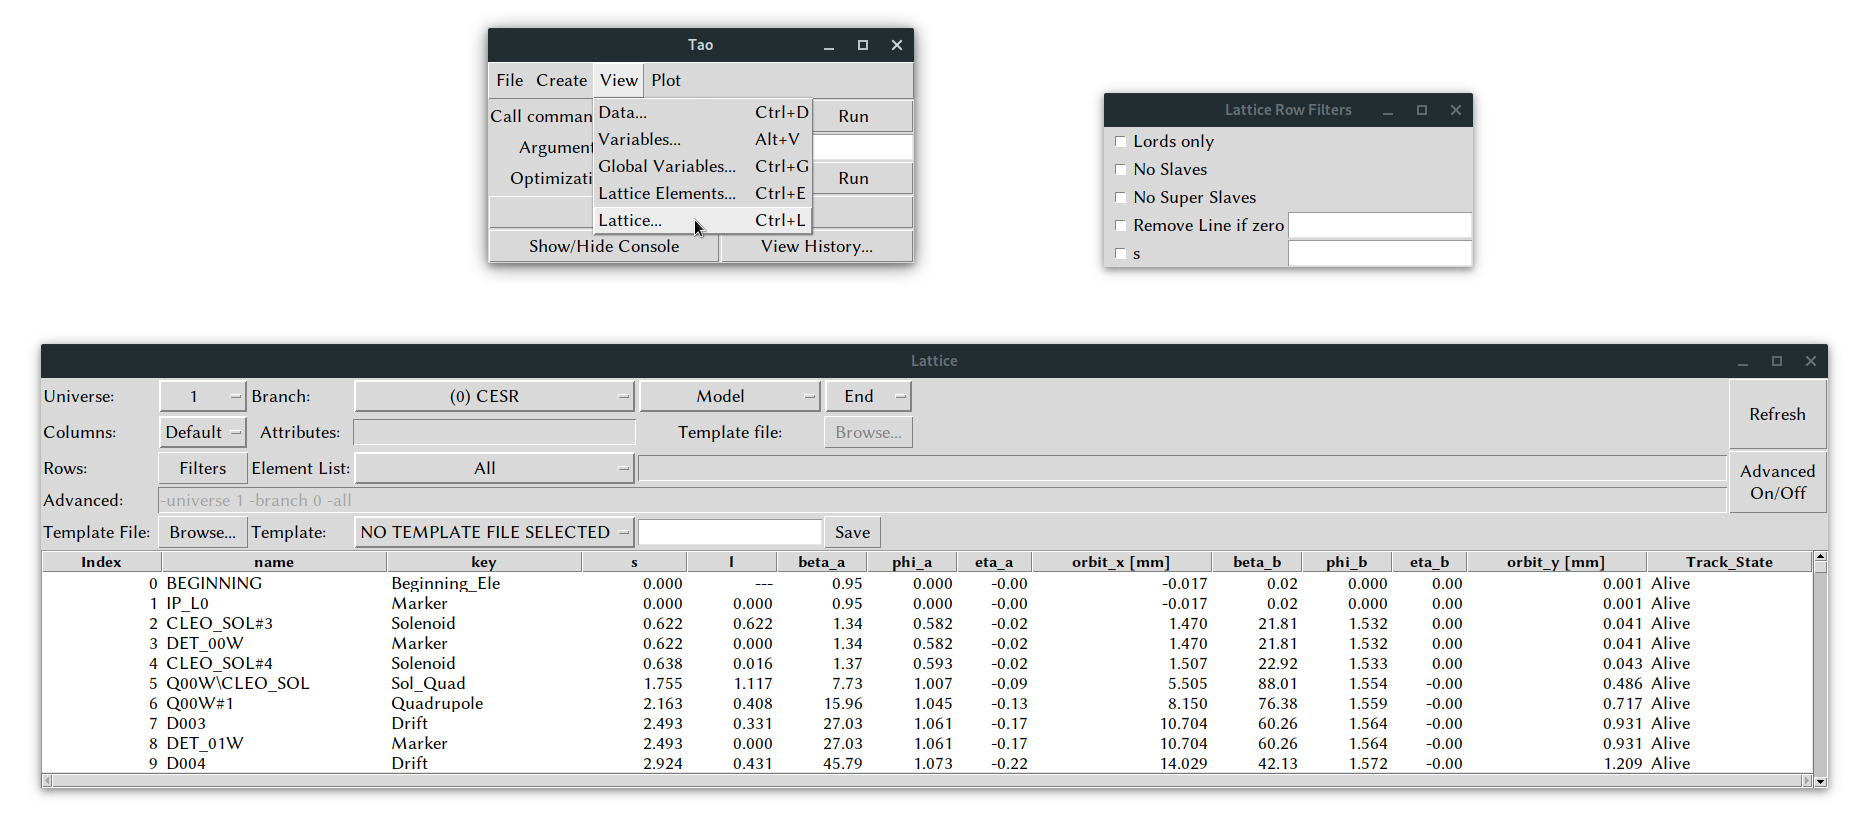
\includegraphics[width=12cm]{figures/lat_table.png}
\caption{The lattice table window.
Top left: accessing the lattice table window from the root window.
Bottom: The lattice table window in its default state.
Top right: the row filter window for the lattice table window.}
\label{fig:gui.lat.table}
\end{figure}
The top portion of the window allows the lattice table to be manipulated, while the bottom portion of the window shows the requested lattice elements and properties.

The first row of settings allows the user to specify the universe and branch of interest, as well as whether base, model, or design parameters should be used, and whether they should be evaluated at the beginning, middle, or end of each element.

The next row allows the user to control what information will be shown in the columns of the table.
Some common presets are available in the drop down menu, but attributes can also be listed manually in the "Attributes" text box.
A lattice template file can also be loaded to determine the column settings (TODO: reference appropriate section in Tao manual).

The next row allows the user to specify which elements will appear in the table.
Clicking on the "Filters" button will open the lattice row filter window (top right in Figure \ref{fig:gui.lat.table}).
The first three settings in this window allow the user to filter in/out the lord and slave elements as desired.
The fourth setting in this window, "Remove line if zero", will filter out any rows that have $0$ in the specified column number.
The final setting in this window allows the user to specify a particular range of s values that elements must have.
Only elements with s within the specified range will be displayed.
The elements to be displayed in the table can also be specified with the "Element List" in the lattice table window.
The user can choose to show all elements, only tracking elements, or a custom list of elements.

The "Advanced" row allows the user to directly set the switches that determine the lattice table, as described in Section (TODO: reference \texttt{show lat} portion of Tao manual).
This box can be toggled on and off with the "Advanced on/off" button to the right of the window.

The final row allows the user to load and save a lattice template file as described in Section \ref{s:gui.lat.templates}.
Loading a template file will populate the template drop-down menu with the defined templates.
The user can also save the current lattice table settings by entering a template name and clicking the "Save button", which will add the new template to the currently open template file.

Once the settings have been adjusted, clicking the "Refresh" button will populate the lattice table according to the specified settings.
The table is scollable, and lists the lord elements at the end of the table if there are any to show.
Double clicking on a row of the table will open an element window for the selected lattice element (see Section \ref{s:gui.lat.elements}).

Figure \ref{fig:gui.lat.table.example} shows an example of the lattice table's capabilities.
\begin{figure}
\centering
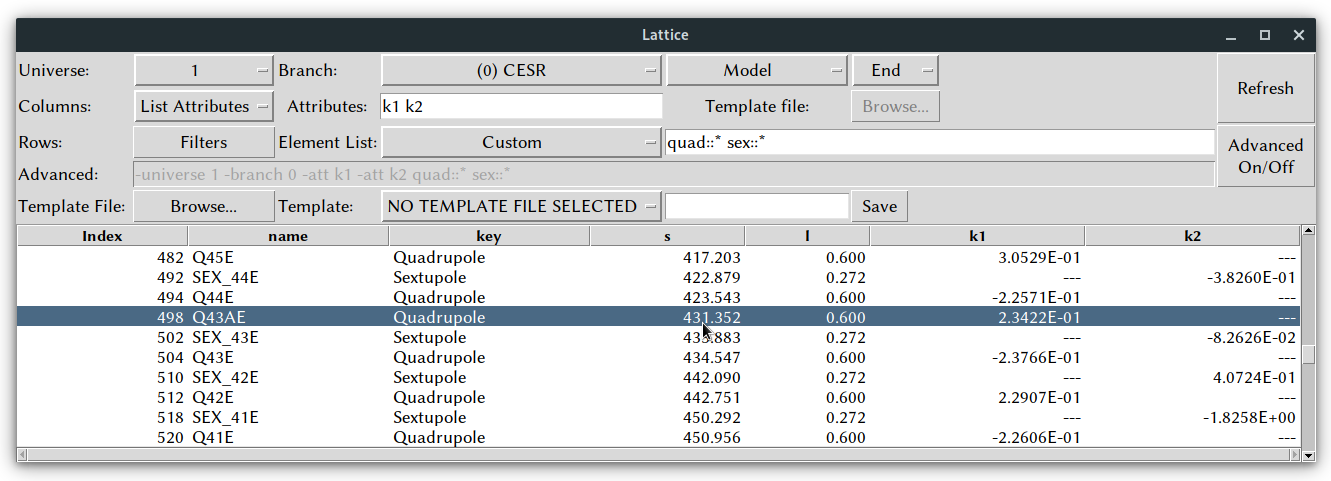
\includegraphics[width=12cm]{figures/lat_table_example.png}
\caption{An example of the lattice table in use.
Here, the table displays all quadrupoles and sextupoles in the lattice, with their k1 and k2 attributes.}
\label{fig:gui.lat.table.example}
\end{figure}
In this example, the user has selected the quadrupole and sextupole elements to be displayed, and has set the k1 and k2 attributes of each element to be shown.

%-----------------------------------------------------------------

\subsection{Lattice Templates}
\label{s:gui.lat.templates}

You can save your settings from the lattice table window in a template file, which can then be loaded and added to from within the gui.
The file can be named anything, and the formatting is as follows:
Lines starting with \# are considered comments and ignored.
Lines starting with "name:" are interpreted as a name for the settings listed in the line directly below
All other lines are interpreted as switches, as would be used with the show lattice command in Tao (see the tao manual for more info).
All switches for a given template should be on one line.

Example:
\begin{example}
#MY TEMPLATE FILE
name:template 1
-orbit -spin -tracking_elements
name:template 2
-lords q*
name: another template
-floor_coords -s 10:20
-radiation_integrals -all
\end{example}

This template file defines four templates: "template 1", "template 2", "another template", and an unnamed template (which has the switches -radiation_integrals -all).  Named templates are displayed by name in the gui, while unnamed templates are simply displayed by what switches they specify.

%-----------------------------------------------------------------
\subsection{Viewing a Lattice Element}
\label{s:gui.lat.elements}

Individual lattice elements can be viewed and editted with the lattice element window as shown in Figure \ref{fig:gui.lat.element.1}.
\begin{figure}
\centering
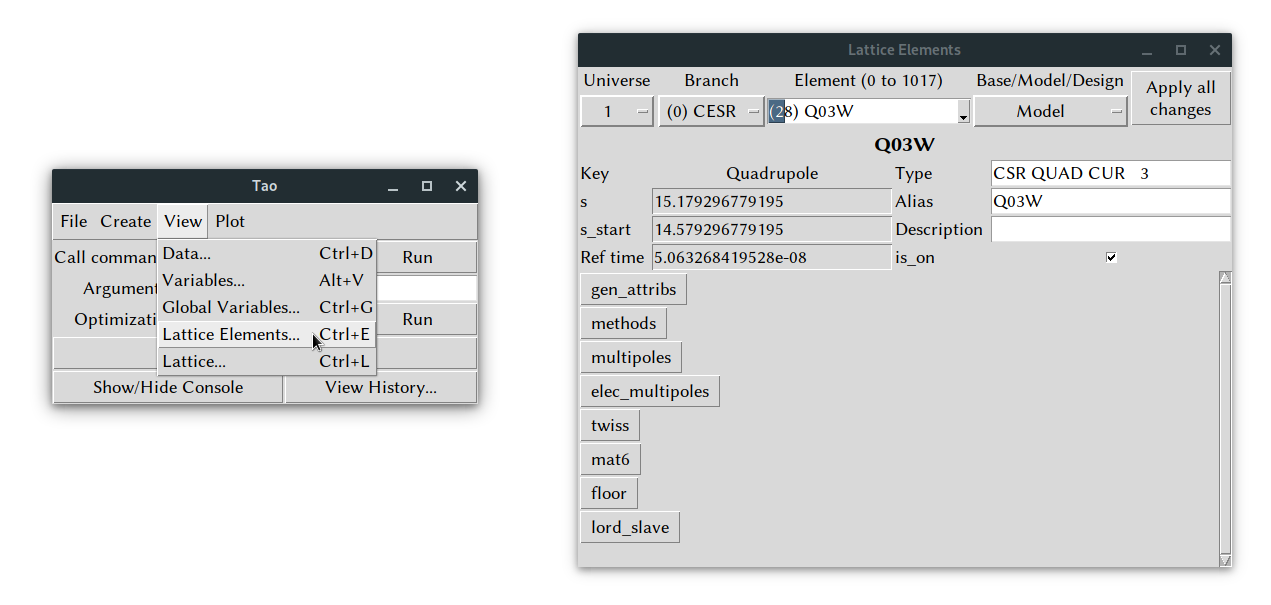
\includegraphics[width=12cm]{figures/lat_element_1.png}
\caption{Accessing the lattice element window.
Here, element Q03W is displayed, with all of its sub-sections collapsed.}
\label{fig:gui.lat.element.1}
\end{figure}
The drop down menus at the top of the window allow the user to select the element to be displayed, as well as whether base, model, or design attributes should be shown.
The next section of the window displays some basic information about the element, some of which can be editted by the user.

The rest of the window is devoted to showing and editting the properties of the selected element.
These properties are divided into sections that can be expanded and collapsed by clicking on the section name.
An example of some of these sections is shown in Figure \ref{fig:gui.lat.element.2}.
\begin{figure}
\centering
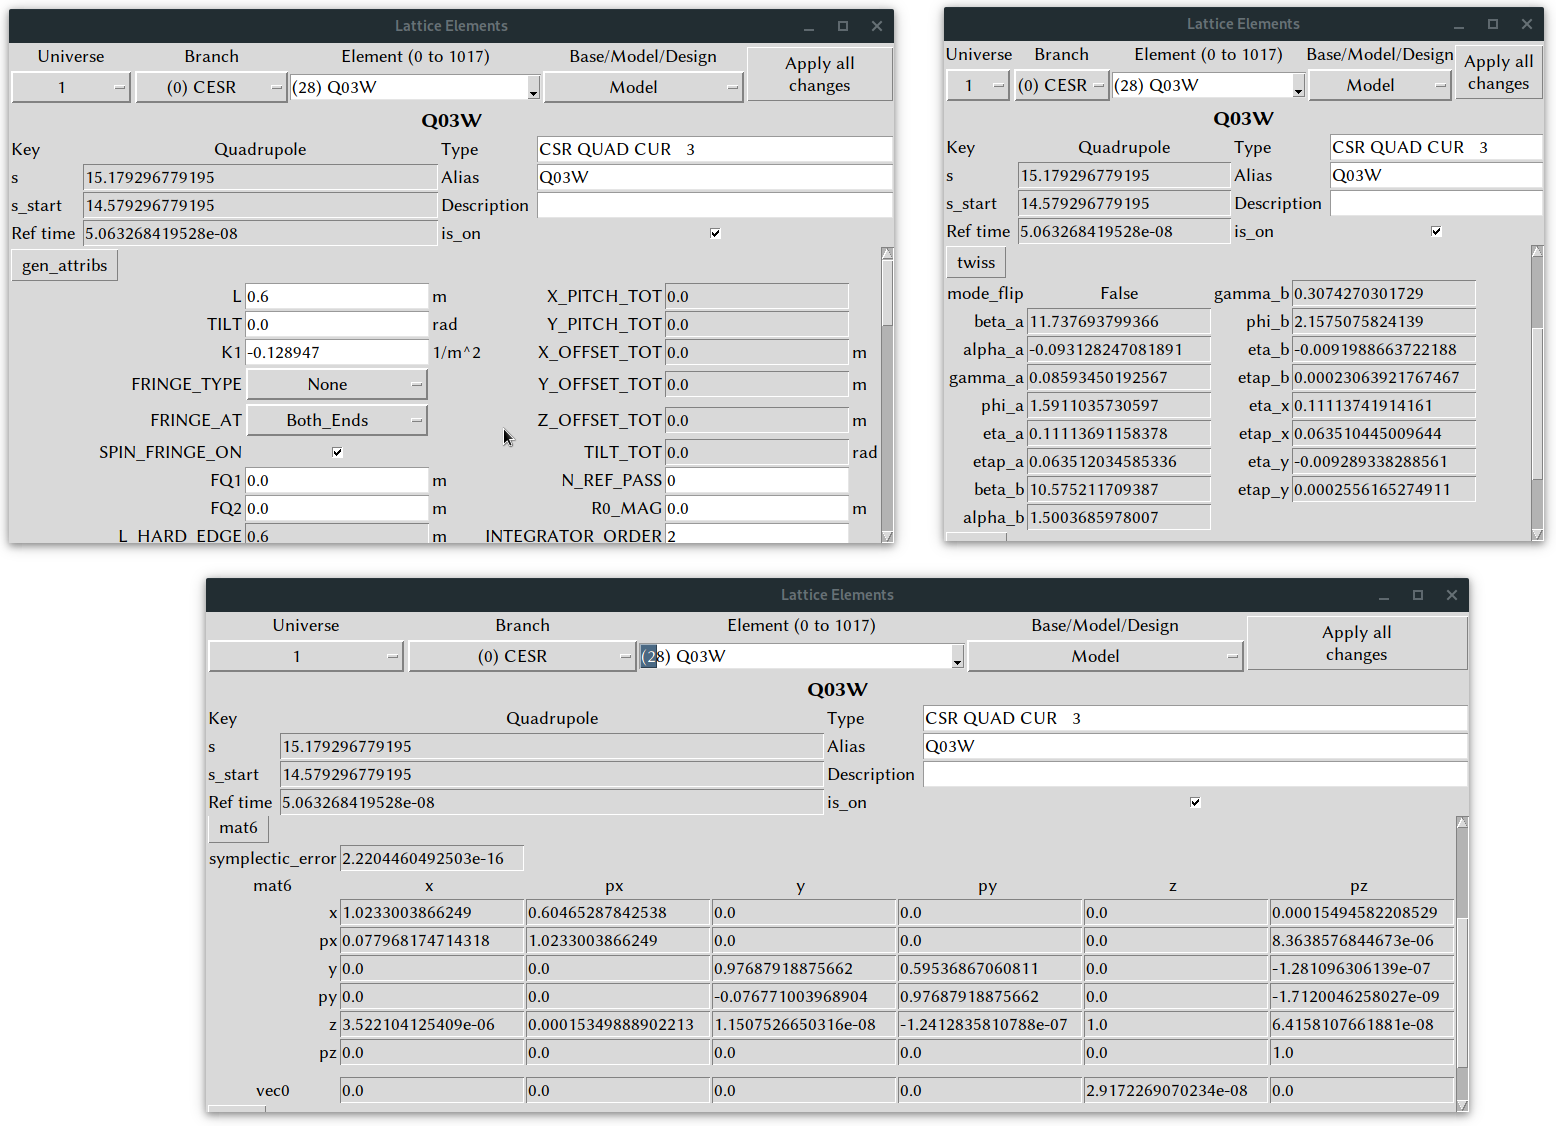
\includegraphics[width=12cm]{figures/lat_element_2.png}
\caption{Some of the collapsable sections of the lattice element window.
Top left: the gen_attribs section.
Top right: the twiss section.
Bottom: the mat6 section.}
\label{fig:gui.lat.element.2}
\end{figure}
Most of the sections display properties in text boxes or drop down menus, some of which can be editted.
There are a few key exceptions to this rule that are listed below.

Elements that have multipoles and/or electric multipoles will have their multipole values displayed in a table under the respective section.
This is shown in Figure \ref{fig:gui.lat.element.multipoles}
\begin{figure}
\centering
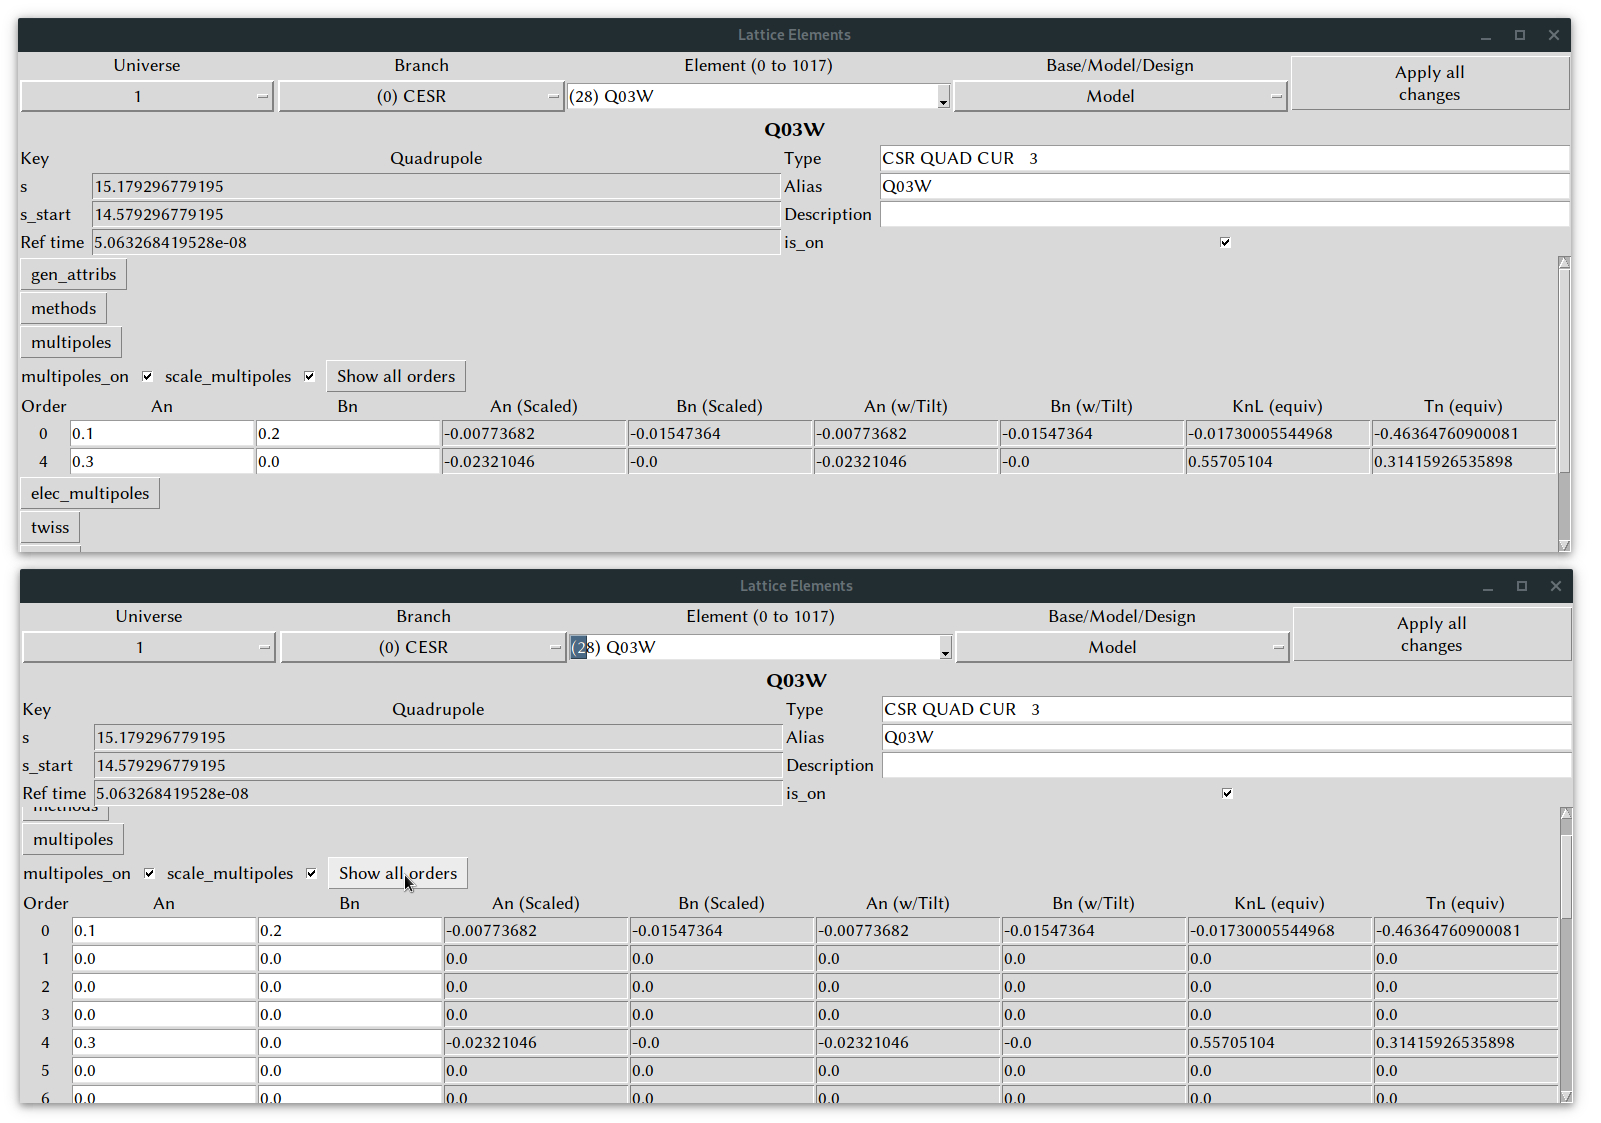
\includegraphics[width=10cm]{figures/lat_element_multipoles.png}
\caption{The magnetic multipoles for Q03W.
Top: by default, only the nonzero multipoles are shown in the table.
Bottom: clicking on the "Show all orders" button will expand the table to allow the user to edit any of the element's multipoles.}
\label{fig:gui.lat.element.multipoles}
\end{figure}
By default, only the orders for which the the multipole is nonzero are shown.
Clicking th3e "Show all orders" button will expand the table to show all multipole orders.
The user can then set the multipole strengths of any order as desired.

The other important exception is the lord_slave section, which displays an element's associated lords and slaves.
For elements that are slaves, this section will list the element's lords in a table.
Clicking on the arrow next to a lord's name will expand a list of that lord's slaves.
Likewise, for a lord element, this section displays a list of the element's slaves.
Clicking on the arrow next to one of these slaves will expand a list of that element's lords.
As with the lattice table, double clicking on an element in the lord/slave list will open another element window for that element.
This is illustrated in Figure \ref{fig:gui.lat.element.lordslave}.
\begin{figure}
\centering
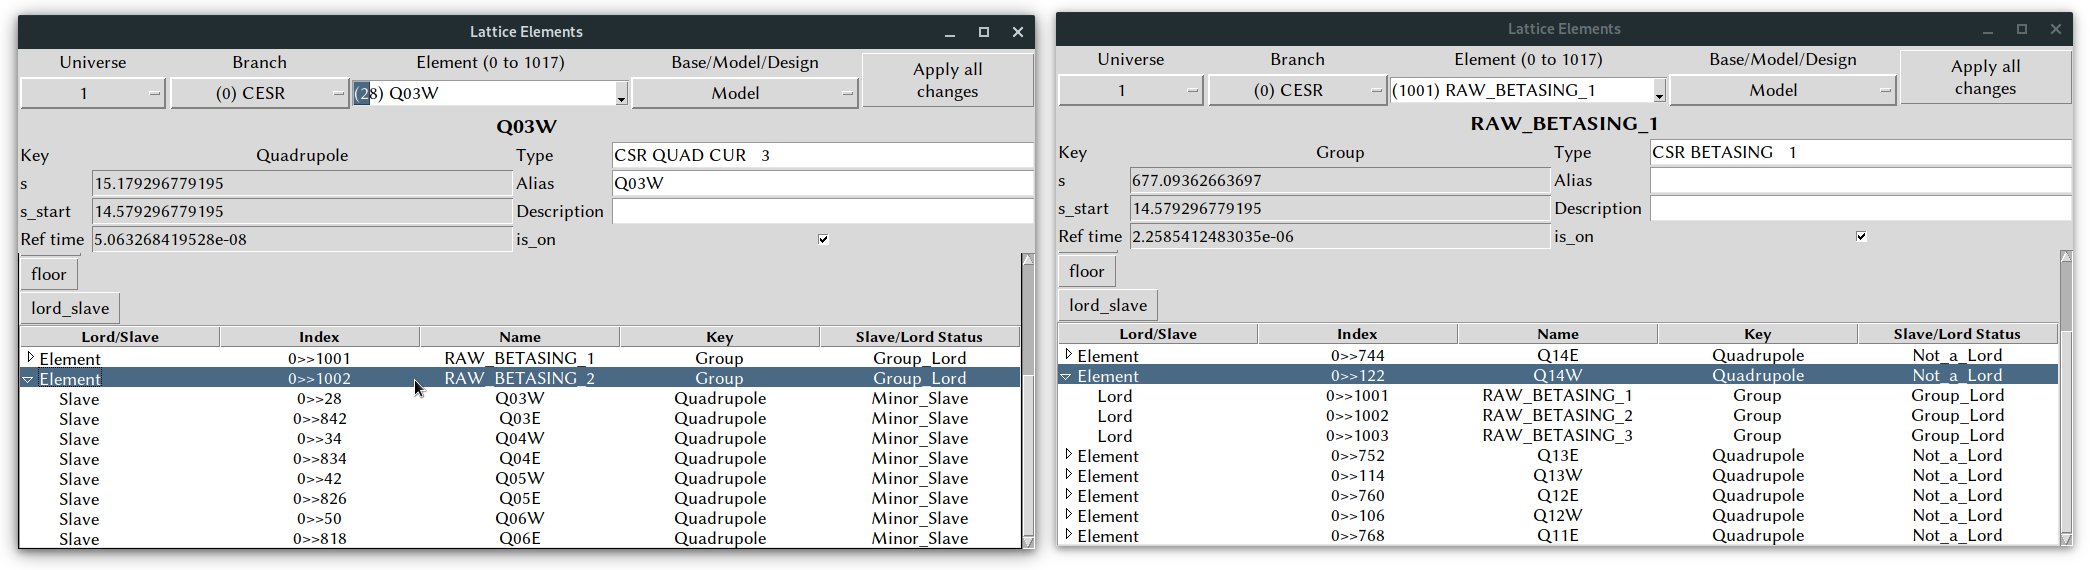
\includegraphics[width=12cm]{figures/lat_lord_slave.png}
\caption{The lord_slave section of the lattice element window.
Left: Q03W is a slave element, and its lords are listed in the table.
One of the lords, RAW_BETASING_2, is expanded to show its slaves.
Right: RAW_BETASING_1 is a lord element, and its slaves are listed in the table.
One of the slaves, Q14W, is expanded to show its lords.}
\label{fig:gui.lat.element.lordslave}
\end{figure}

Once the information in each section has been modified as needed, clicking the "Apply all changes" button will change the element properties in Tao.
